\subsection{FLV Graphs}\label{subsec:flvGraphs}
The beneath diagram shows the 4 fuzzy linguistic variables for a gazelle.
These follow the rules of the next subsection.
As you can see, there is two factors a gazelle can use in order to determine if it wants to run or it wants to eat.
We also implemented fuzzy logic for the lion, but we will not describe it in this document.
\begin{figure}[ht]
    \begin{center}
        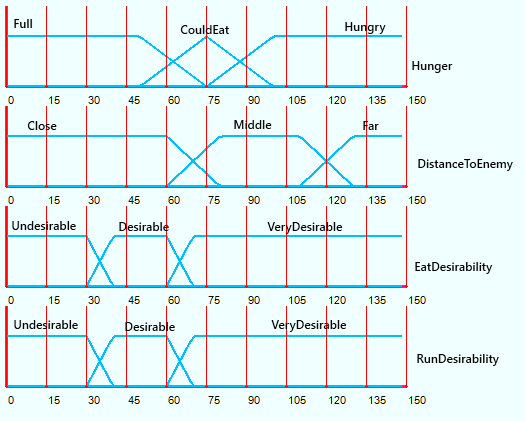
\includegraphics[width=25em]{FuzzyLogic.PNG}
    \end{center}
    \caption{Fuzzy logic explanation}
    \label{fig:FuzzyLogicExplanation}
\end{figure}
\subsection{Rulesets}
These are the rulesets used in our program.
They only portray the two decisions of a gazelle, namely wanna eat and wanna run.
The horizontal values (close, middle and far) are aimed at the distance between the gazelle and a lion.
The vertical values (full, couldeat and hungry) are aimed at the hunger the gazelle experiences.
Based on these values, the gazelle should be able to choose if gathering food is undesirable, desirable or verydesirable.
\begin{table}[ht]
    \centering
    \label{EatDesirability}
    \begin{tabular}{|l|l|l|l|}
        \hline
        & \textbf{Close}       & \textbf{Middle}        & \textbf{Far}           \\ \hline
        \textbf{Full}     & Undesirable & Undesirable   & Desirable     \\ \hline
        \textbf{CouldEat} & Undesirable & Desirable     & VeryDesirable \\ \hline
        \textbf{Hungry}   & Undesirable & VeryDesirable & VeryDesirable \\ \hline
    \end{tabular}
    \caption{GazelleWannaEat}
\end{table}
\begin{table}[ht]
    \centering
    \label{|RunDesirability}
    \begin{tabular}{|l|l|l|l|}
        \hline
        & \textbf{Close}       & \textbf{Middle}        & \textbf{Far}           \\ \hline
        \textbf{Full}     & VeryDesirable & VeryDesirable   & Undesirable     \\ \hline
        \textbf{CouldEat} & VeryDesirable & Desirable     & Undesirable \\ \hline
        \textbf{Hungry}   & VeryDesirable & Desirable & Undesirable \\ \hline
    \end{tabular}
    \caption{GazelleWannaRun}
\end{table}
\subsection{Calculation}\label{subsec:calculation}
In this section I will do two calculations, to show how the fuzzy logic works, and how it works with our implementation.
For the first situation we pick two variables for the antecedents, namely 140 for the DistanceToEnemy and 80 for the Hunger.
\begin{figure}[ht]
    \begin{center}
        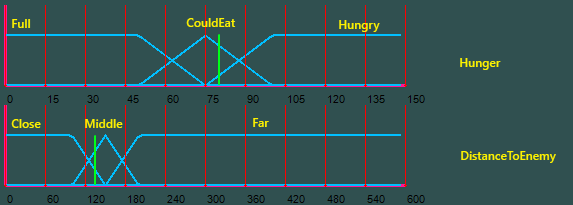
\includegraphics[width=20em]{FuzzyLogicCaseOne.PNG}
    \end{center}
    \caption{Fuzzy logic case 1}
    \label{fig:FuzzyLogicCaseOne}
\end{figure}
As you see, we drew a line on the value of 80 in the Hunger FLV, and a line on the value of 140 on the DistanceToEnemy FLV\@.
Right now, we can determine that for the first flv:
{\em Full(80)} is {\em 0} \\
{\em CouldEat(80)} is approx {\em  0.8} \\
{\em Hungry(80)} is approx {\em 0.2} \\
And for the second FLV:
{\em Close(140)} is {\em 0.2} \\
{\em Middle(140)} is approx {\em 0.8} \\
{\em Far(140)} is approx {\em 0} \\
Now, for both consequents we can fill in the table.
\begin{table}[ht]
    \centering
    \label{EatDesirabilityCaseOne}
    \begin{tabular}{|l|l|l|l|}
        \hline
        & \textbf{Close}    & \textbf{Middle}     & \textbf{Far}           \\ \hline
        \textbf{Full}     & Undesirable (0)   & Undesirable   (0)   & Desirable     (0) \\ \hline
        \textbf{CouldEat} & Undesirable (0.2) & Desirable     (0.8) & VeryDesirable (0) \\ \hline
        \textbf{Hungry}   & Undesirable (0.2) & VeryDesirable (0.2) & VeryDesirable (0) \\ \hline
    \end{tabular}
    \caption{EatDesirability}
\end{table}
\begin{table}[ht]
    \centering
    \label{RunDesirabilityCaseOne}
    \begin{tabular}{|l|l|l|l|}
        \hline
                          & \textbf{Close}      & \textbf{Middle}     & \textbf{Far}\\ \hline
        \textbf{Full}     & VeryDesirable (0)   & VeryDesirable (0)   & Undesirable (0) \\ \hline
        \textbf{CouldEat} & VeryDesirable (0.2) & Desirable     (0.8) & Undesirable (0) \\ \hline
        \textbf{Hungry}   & VeryDesirable (0.2) & Desirable     (0.2) & Undesirable (0) \\ \hline
    \end{tabular}
    \caption{RunDesirability}
\end{table}
This can be calculated into a max value for all FuzzySets.
\begin{table}[ht]
    \centering
    \label{InferedConclusionsEatDesirability}
    \begin{tabular}{|l|l|}
        \hline
        \textbf{Undesirable}   & 0.2 \\ \hline
        \textbf{Desirable}     & 0.8 \\ \hline
        \textbf{VeryDesirable} & 0.2 \\ \hline
    \end{tabular}
    \caption{Infered conclusions EatDesirability}
\end{table}
\begin{table}[ht]
    \centering
    \label{InferedConclusionsRunDesirability}
    \begin{tabular}{|l|l|}
        \hline
        \textbf{Undesirable}   & 0.2   \\ \hline
        \textbf{Desirable}     & 0.8 \\ \hline
        \textbf{VeryDesirable} & 0.3 \\ \hline
    \end{tabular}
    \caption{Infered conclusions RunDesirability}
\end{table}
Now we have these infered conclusions, we can defuzzify the consequents!
We will use MaxAV, since MaxAV is mainly used in our program.
Also, centroid is implemented, but we wont discuss that in this documentation.
For this, we have to calculate the maxima of both consequent FLV's.
You can check this in the graph above, right now I just took the values we chose to draw the graphs.
In the EatDesirability consequent, the maxima are:
\begin{equation}
    Eat_{Undesirable} = \frac{0 + 10}2 = 5
\end{equation}
\begin{equation}
    Eat_{Desirable} = \frac{20 + 50}2 = 35
\end{equation}
\begin{equation}
    Eat_{VeryDesirable} = \frac{60 + 150}2 = 105
\end{equation}
And now defuzzify with MaxAV through the following formula:
\begin{equation}
    MaxAV = \frac{5 * 0.2 + 35 * 0.8 + 105 * 0.2}{0.2 + 0.8 + 0.2} = 41.7
\end{equation}
In the RunDesirability consequent, the maxima are:
\begin{equation}
    Run_{Undesirable} = \frac{0 + 10}2 = 5
\end{equation}
\begin{equation}
    Run_{Desirable} = \frac{20 + 30}2 = 25
\end{equation}
\begin{equation}
    Run_{VeryDesirable} = \frac{50 + 150}2 = 100
\end{equation}
And now defuzzify with MaxAV through the following formula:
\begin{equation}
    MaxAV = \frac{5 * 0.2 + 25 * 0.8 + 100 * 0.3}{0.2 + 0.8 + 0.3} = 39.2
\end{equation}

\newpage
\subsection{Code fragment}
Right now we will do the exact calculation as above, but then with our code.
First, we will create a fuzzy module with two antecedents.
\begin{figure}[ht]
    \begin{center}
        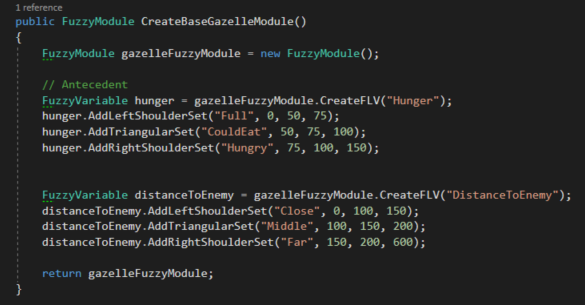
\includegraphics[width=40em]{FuzzyModuleGazelle.PNG}
    \end{center}
    \caption{Fuzzy module gazelle}
    \label{fig:FuzzyModuleGazelle}
\end{figure}
Then, we will create two consequents with its own rulesets, namely WannaRun and WannaEat, as following!
\newpage
\begin{figure}[ht]
    \begin{center}
        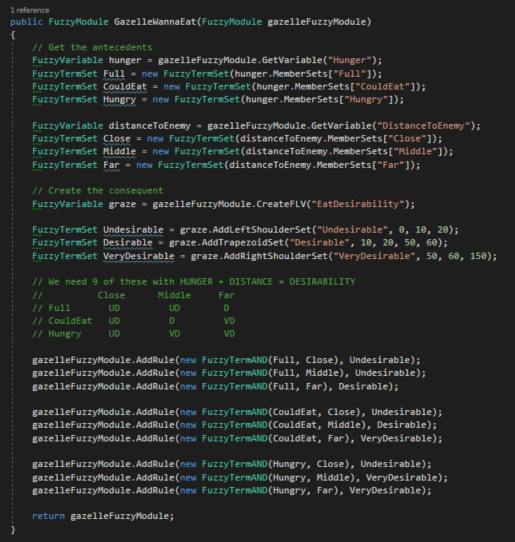
\includegraphics[width=40em]{FuzzyWannaEat.PNG}
    \end{center}
    \caption{Fuzzy wanna eat consequence + ruleset}
    \label{fig:FuzzyWannaEat}
\end{figure}
In this figure you see firstly we get all the variables from our already created module and create new TermSets so we can use them in our rules.
Next, we create a FLV according to the values of this module.
The values inside the AddLeftShoulderSet are predefined, and you can just adjust them if you want to have a different result.
Then, we add all the rules.
In comments we created a visual overview of the ruleset.
This is exactly the same as the rules added to the fuzzy module.
\newpage
\begin{figure}[ht]
    \begin{center}
        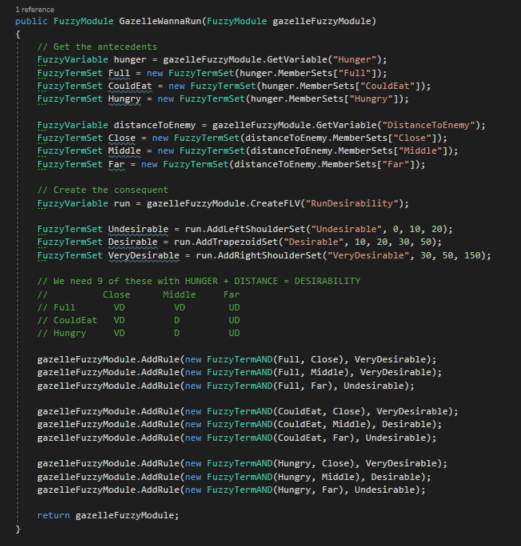
\includegraphics[width=40em]{FuzzyWannaRun.PNG}
    \end{center}
    \caption{Fuzzy wanna run consequence + ruleset}
    \label{fig:FuzzyWannaRun}
\end{figure}
Everything is exactly the same as the above, but with different values and a different ruleset.
Pretty neat and easy, right?
\newpage
\subsection{Class diagram}
\begin{figure}[ht]
    \begin{center}
        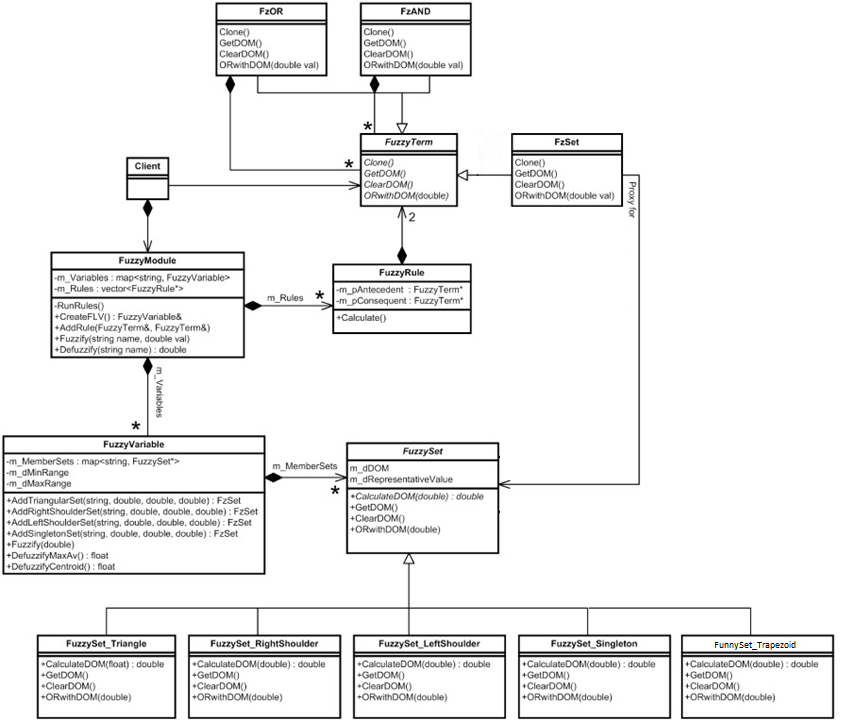
\includegraphics[width=35em]{FuzzyClassDiagram.png}
    \end{center}
    \begin{center}
    \caption{Fuzzy logic class diagram}
    \\Note: This is imported and edited from the following book \cite{pgaie} %TODO: Should be fixed so reference works.
    \end{center}
    \label{fig:FuzzyClassDiagram}
\end{figure}
\newpage
\newpage
%-----------------------------------------------------------------------------------------